\documentclass[11pt]{article}
\usepackage[lmargin=1in,rmargin=1.75in,bmargin=1in,tmargin=1in]{geometry}

% For hyperlinking everything
\usepackage{hyperref}
\hypersetup{
	colorlinks=true, %set true if you want colored links
	linktoc=all,     %set to all if you want both sections and subsections linked
	linkcolor=blue,  %choose some color if you want links to stand out
}


\usepackage[latin1]{inputenc}
\usepackage{amsmath}
\usepackage{mathrsfs}  
\usepackage{amsfonts}
\usepackage{amssymb}
\usepackage{graphicx}
\usepackage{subfig}
\usepackage{caption}
\usepackage{algorithm}
%\usepackage{algcompatible}
%\usepackage{algorithmicx}
\usepackage{algpseudocode}

\usepackage{titlesec}
\titleformat{\section}{\fontfamily{lmss}\fontsize{14}{15}\bfseries}{\thesection}{1em}{}
\titleformat{\subsection}{\fontfamily{lmss}\fontsize{12}{15}\bfseries}{\thesubsection}{1em}{}




\usepackage{amsthm}

\newtheoremstyle{noit}
{10pt}% <Space above>
{10pt}% <Space below>
{}% <Body font>
{}% <Indent amount>
{\bfseries}% <Theorem head font>
{.}% <Punctuation after theorem head>
{.5em}% <Space after theorem headi>
{}% <Theorem head spec (can be left empty, meaning `normal')>

\newtheoremstyle{example}
{10pt}% <Space above>
{10pt}% <Space below>
{}% <Body font>
{20pt}% <Indent amount>
{\bfseries}% <Theorem head font>
{.}% <Punctuation after theorem head>
{.5em}% <Space after theorem headi>
{}% <Theorem head spec (can be left empty, meaning `normal')>


\newtheoremstyle{indented}{20pt}{20pt}{\addtolength{\leftskip}{2.5em}}{}{\bfseries}{.}{.5em}{}


\newtheorem{theorem}{Theorem}
\numberwithin{theorem}{section}
\newtheorem{lemma}[theorem]{Lemma}
\newtheorem{corollary}[theorem]{Corollary}
\newtheorem{observation}{Observation}
%\numberwithin{observation}{section}
%\numberwithin{definition}{section}
\newtheorem{conjecture}{Conjecture}
\newtheorem{Qu}{Question}
\newcommand{\QU}{\begin{Qu}\normalfont}

\theoremstyle{noit}
\newtheorem{fact}{Fact}
\newtheorem{definition}{Definition}

\theoremstyle{indented}
\newtheorem{example}{Example}

\theoremstyle{indented}
\newtheorem{problem}{Problem}


%\newenvironment{proof}{\noindent{\bf Proof:} \hspace*{1em}}{
%    \hspace*{\fill} $\Box$ }
%\newenvironment{proof_of}[1]{\noindent {\bf Proof of #1:}
%    \hspace*{1em} }{\hspace*{\fill} $\Box$ }
%\newenvironment{proof_claim}{\begin{quotation} \noindent}{
%    \hspace*{\fill} $\diamond$ \end{quotation}}
\newcommand{\vs}[1]{\vspace{#1}}

\newcommand{\lecture}[2]{
 \noindent
\begin{center}
	\framebox{
		\vbox{
			\hbox to 5.78in { {\bf CSCE 411: Design and Analysis of Algorithms (Honors)} \hfill  }
			\vspace{2mm}
			\hbox to 5.78in { {\Large \hfill Lecture #1\hfill} }
			\vspace{2mm}
			\hbox to 5.78in { {\it Date: #2 \hfill Samson Zhou} }
		}
	}
\end{center}
\vspace*{4mm}
}

\newcommand{\week}[2]{
 \noindent
\begin{center}
	\framebox{
		\vbox{
			\hbox to 5.78in { {\bf CSCE 411: Design and Analysis of Algorithms (Honors)} \hfill  }
			\vspace{2mm}
			\hbox to 5.78in { {\Large \hfill Week #1\hfill} }
			\vspace{2mm}
			\hbox to 5.78in { {\it Date: #2 \hfill Nate Veldt, updated by Samson Zhou} }
		}
	}
\end{center}
\vspace*{4mm}
}

\newcommand{\sweek}[2]{
 \noindent
\begin{center}
	\framebox{
		\vbox{
			\hbox to 5.78in { {\bf CSCE 411: Design and Analysis of Algorithms (Honors)} \hfill  }
			\vspace{2mm}
			\hbox to 5.78in { {\Large \hfill Week #1\hfill} }
			\vspace{2mm}
			\hbox to 5.78in { {\it Date: #2 \hfill Samson Zhou} }
		}
	}
\end{center}
\vspace*{4mm}
}

\newcommand{\hw}[2]{
	\noindent
	\begin{center}
		\framebox{
			\vbox{
				\hbox to 5.78in { {\bf CSCE 411: Design and Analysis of Algorithms} \hfill  }
				\vspace{2mm}
				\hbox to 5.78in { {\Large \hfill Homework #1\hfill} }
				\vspace{2mm}
				\hbox to 5.78in { {\it Due date: #2 \hfil} }
			}
		}
	\end{center}
	\vspace*{4mm}
}



\newcommand{\under}[1]{\underline{\hspace{#1}}}
\setlength{\parindent}{0em}

%\usepackage[tagged]{accessibility}

% Graph terms
\newcommand{\vol}{\textbf{vol}}
\newcommand{\cut}{\textbf{cut}}


% Matrices
\newcommand{\mA}{\textbf{A}}
\newcommand{\mB}{\textbf{B}}

% vectors
\newcommand{\ve}{\textbf{e}}
\newcommand{\vx}{\textbf{x}}


% Other
\newcommand{\calN}{\mathcal{N}}

\usepackage{mathtools}
\DeclarePairedDelimiter\ceil{\lceil}{\rceil}
\DeclarePairedDelimiter\floor{\lfloor}{\rfloor}


\newcommand*{\aitem}{ \item[{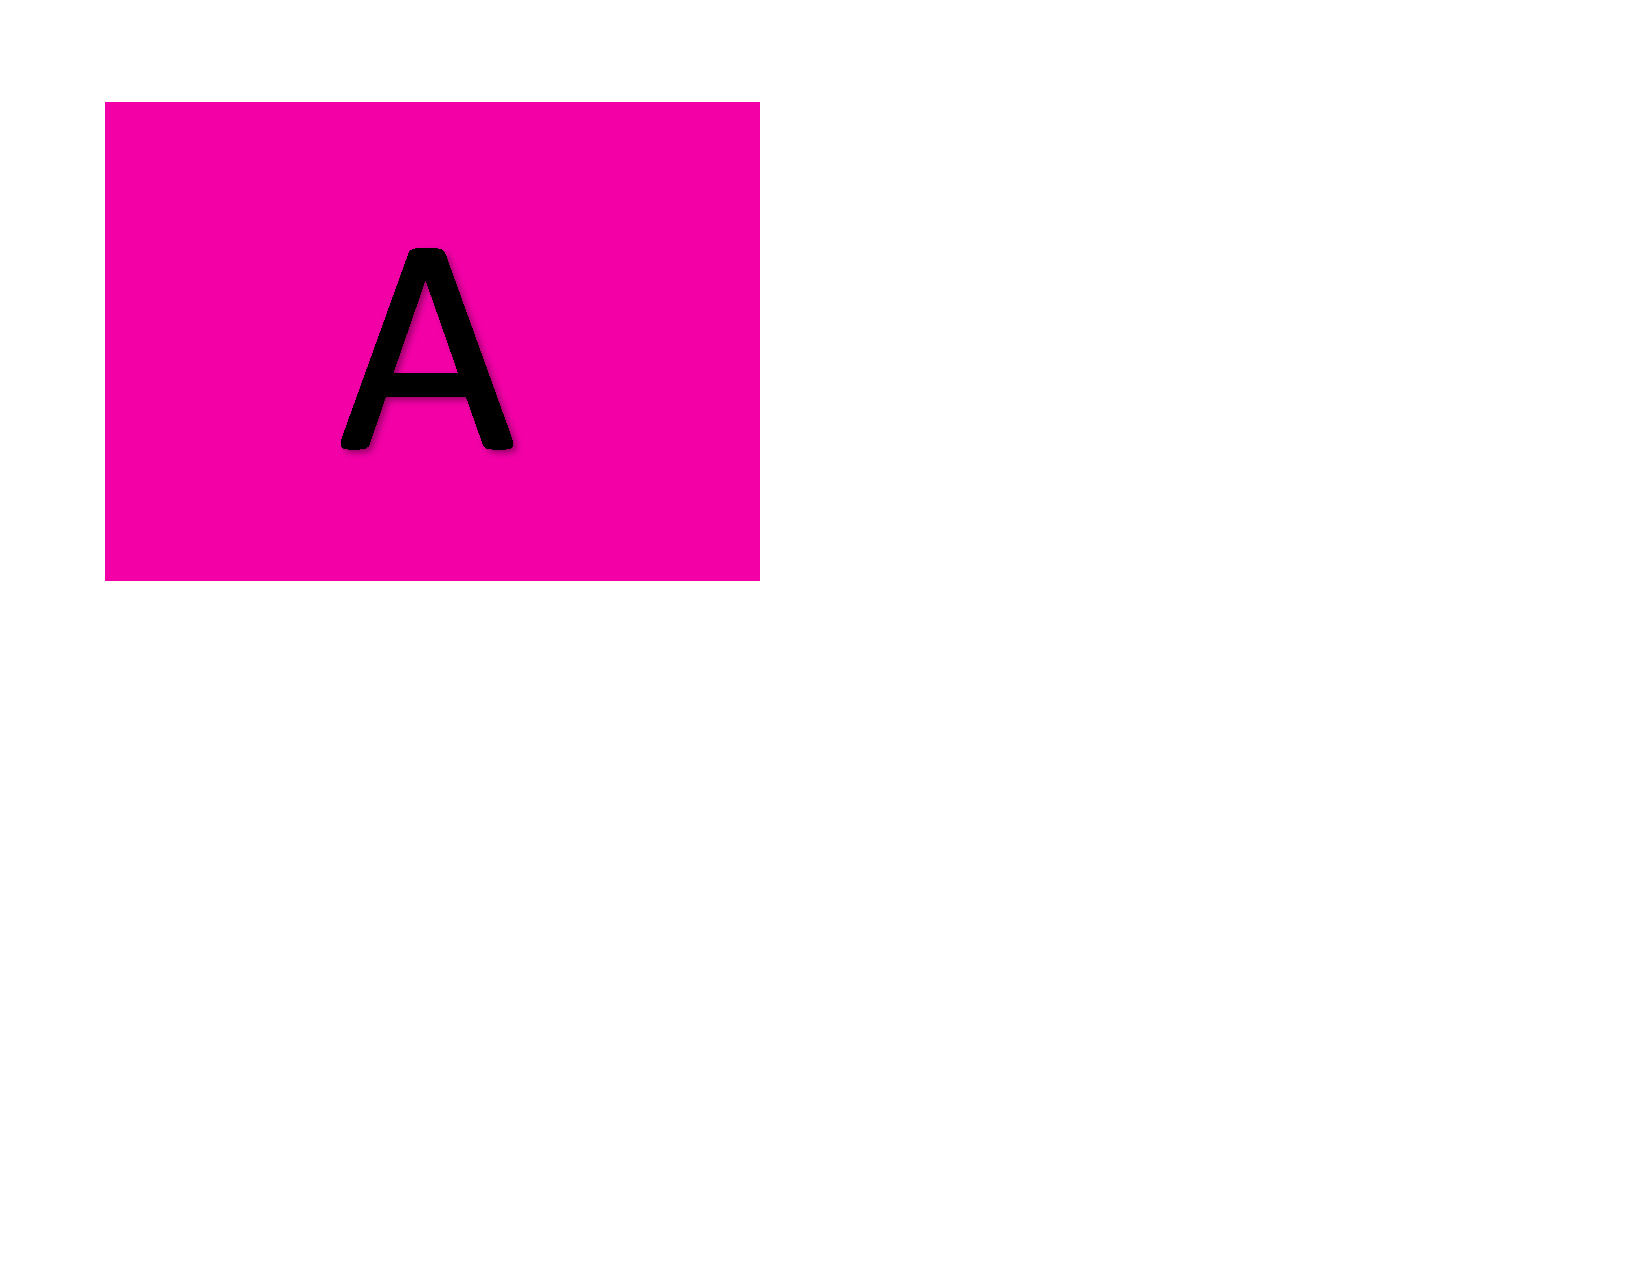
\includegraphics[width=0.8cm,height=0.5cm]{figures/A}} ]  }
\newcommand*{\bitem}{ \item[{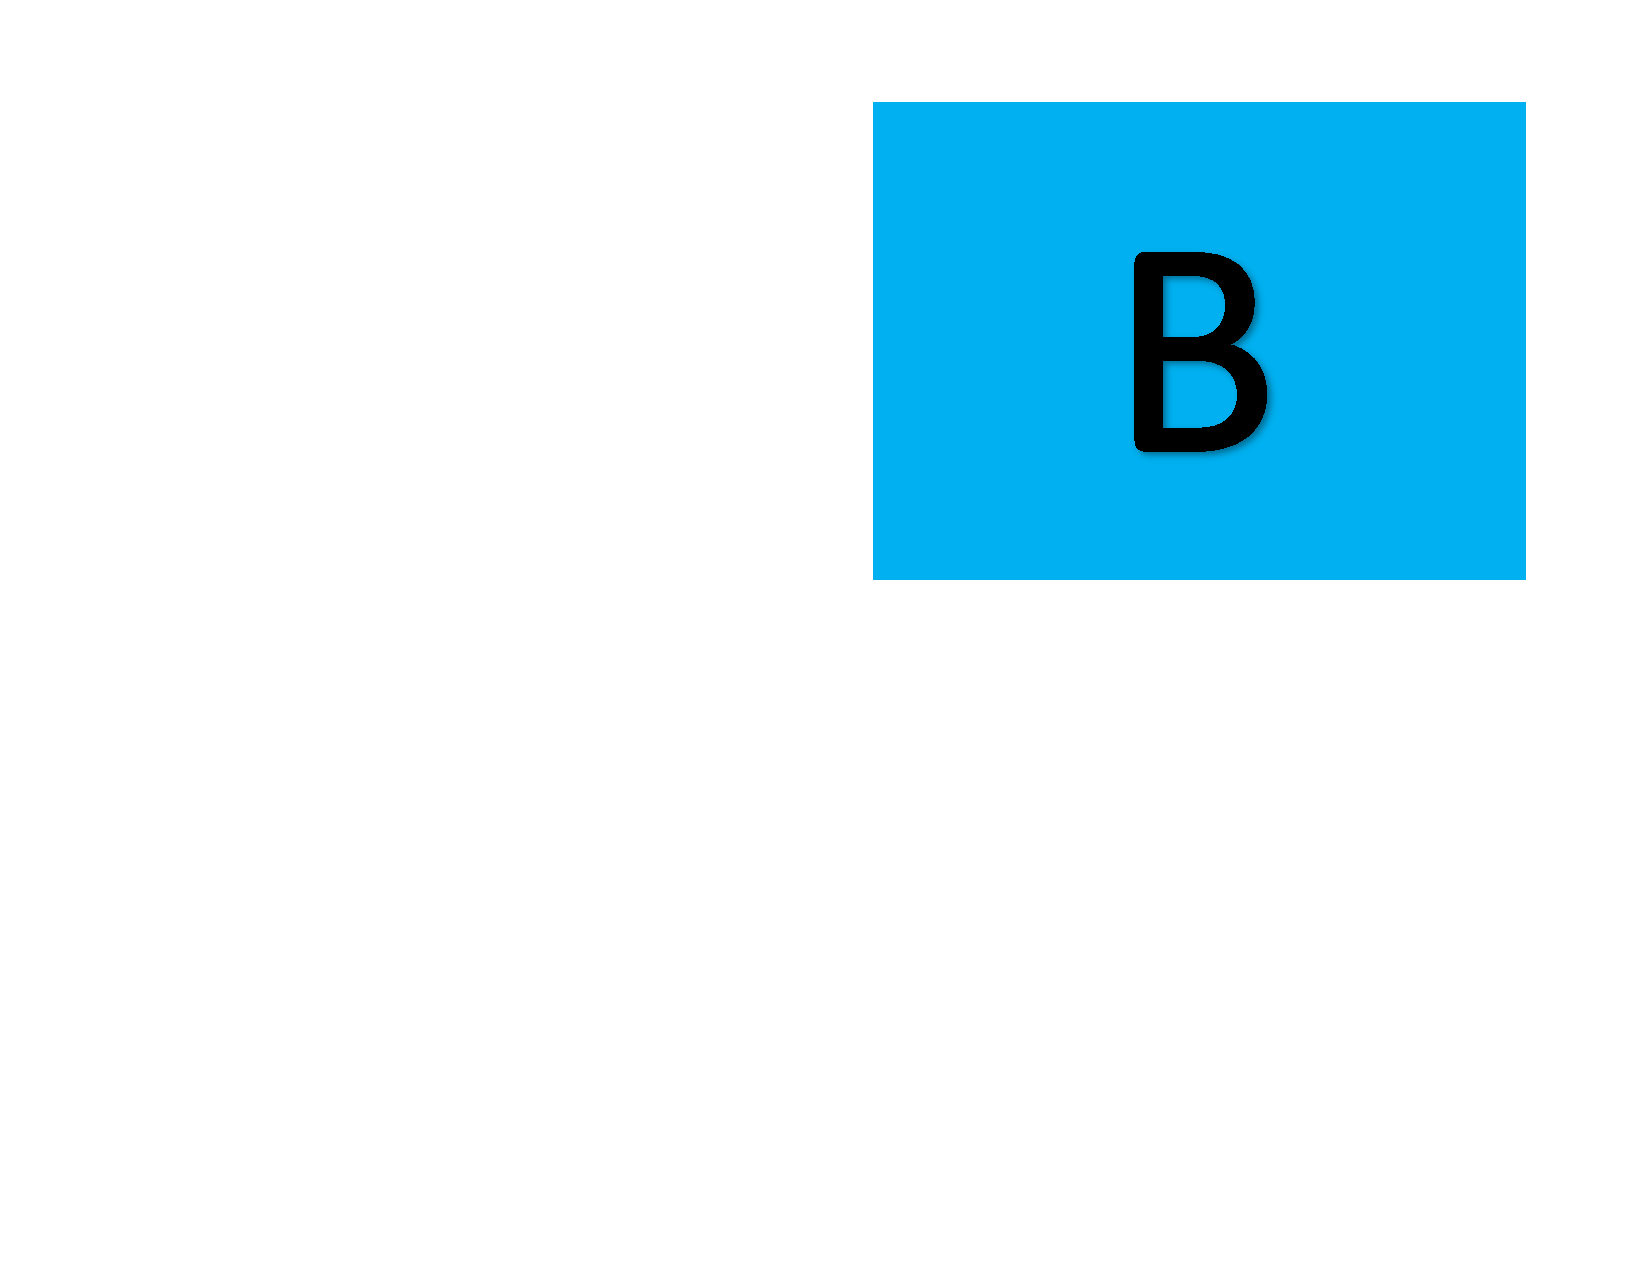
\includegraphics[width=0.8cm,height=0.5cm]{figures/B}} ]  }
\newcommand*{\citem}{ \item[{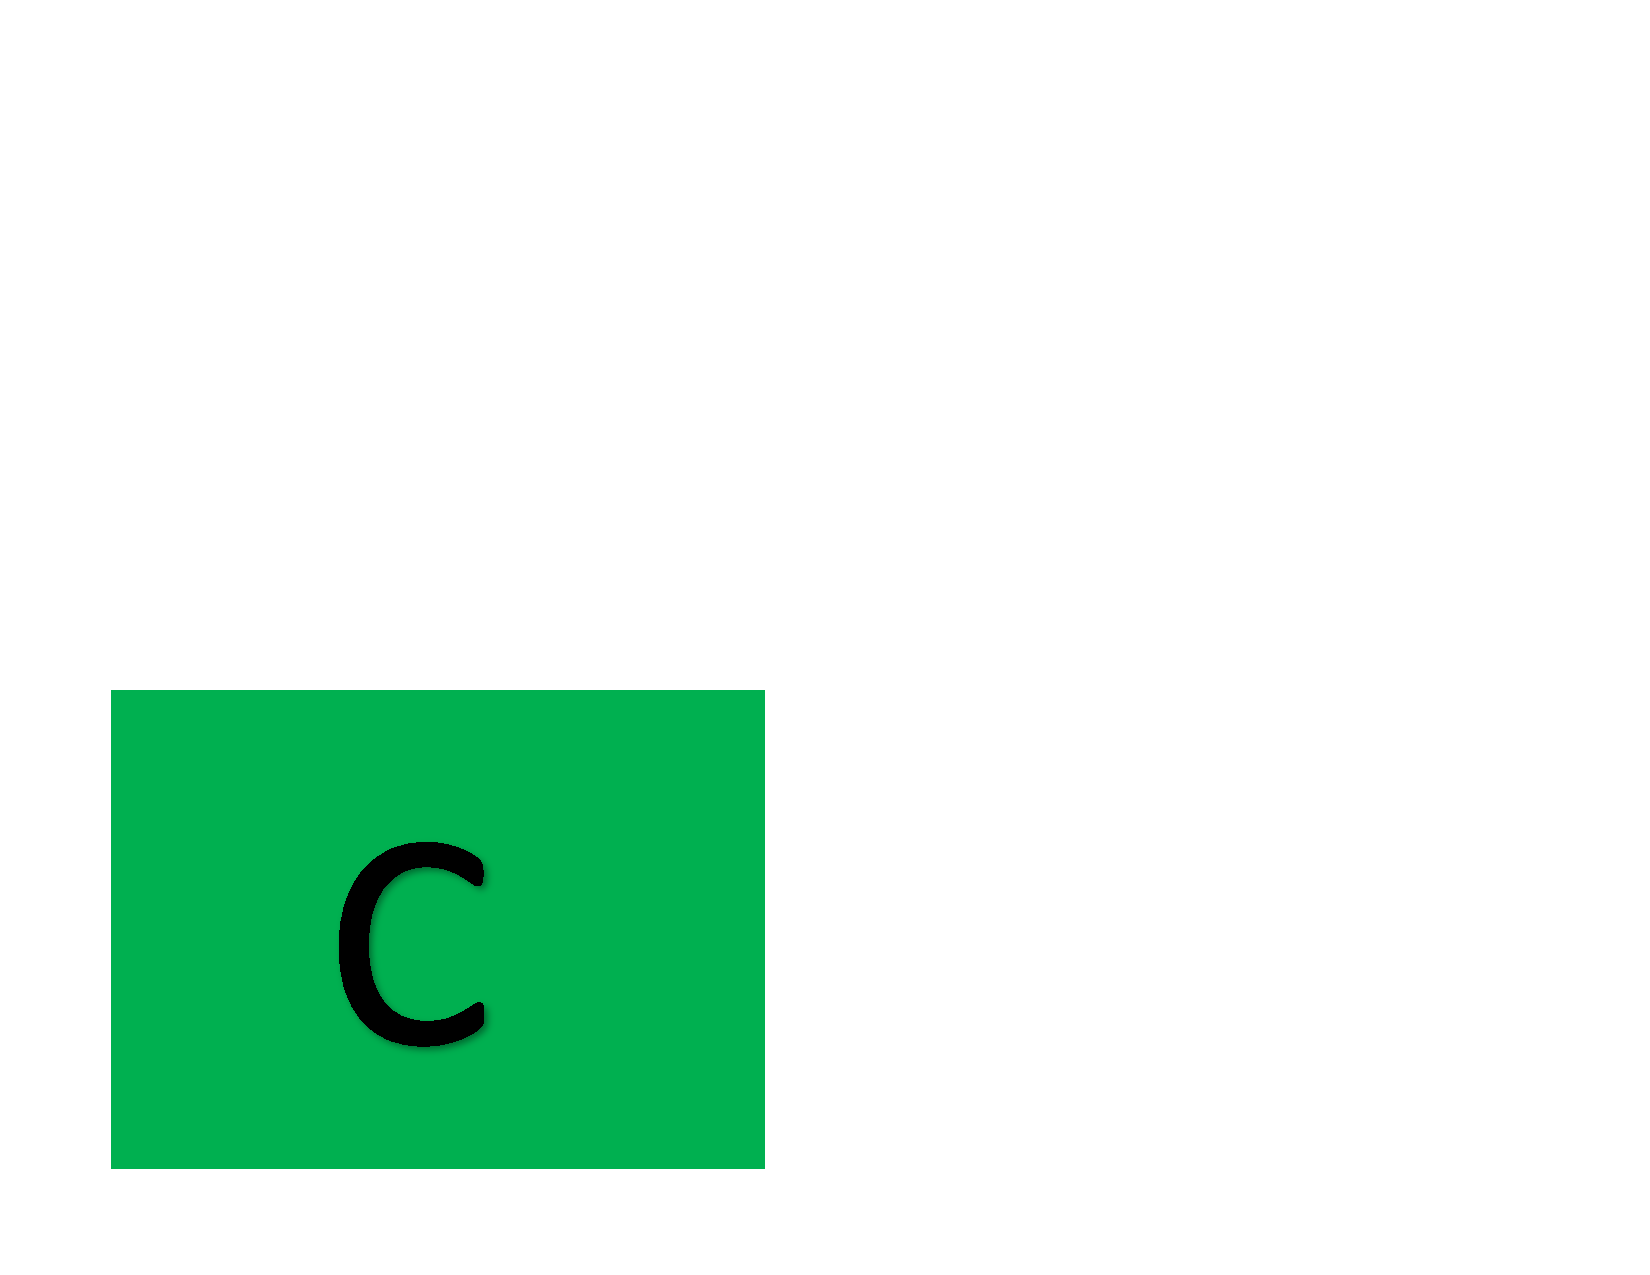
\includegraphics[width=0.8cm,height=0.5cm]{figures/C}} ]  }
\newcommand*{\ditem}{ \item[{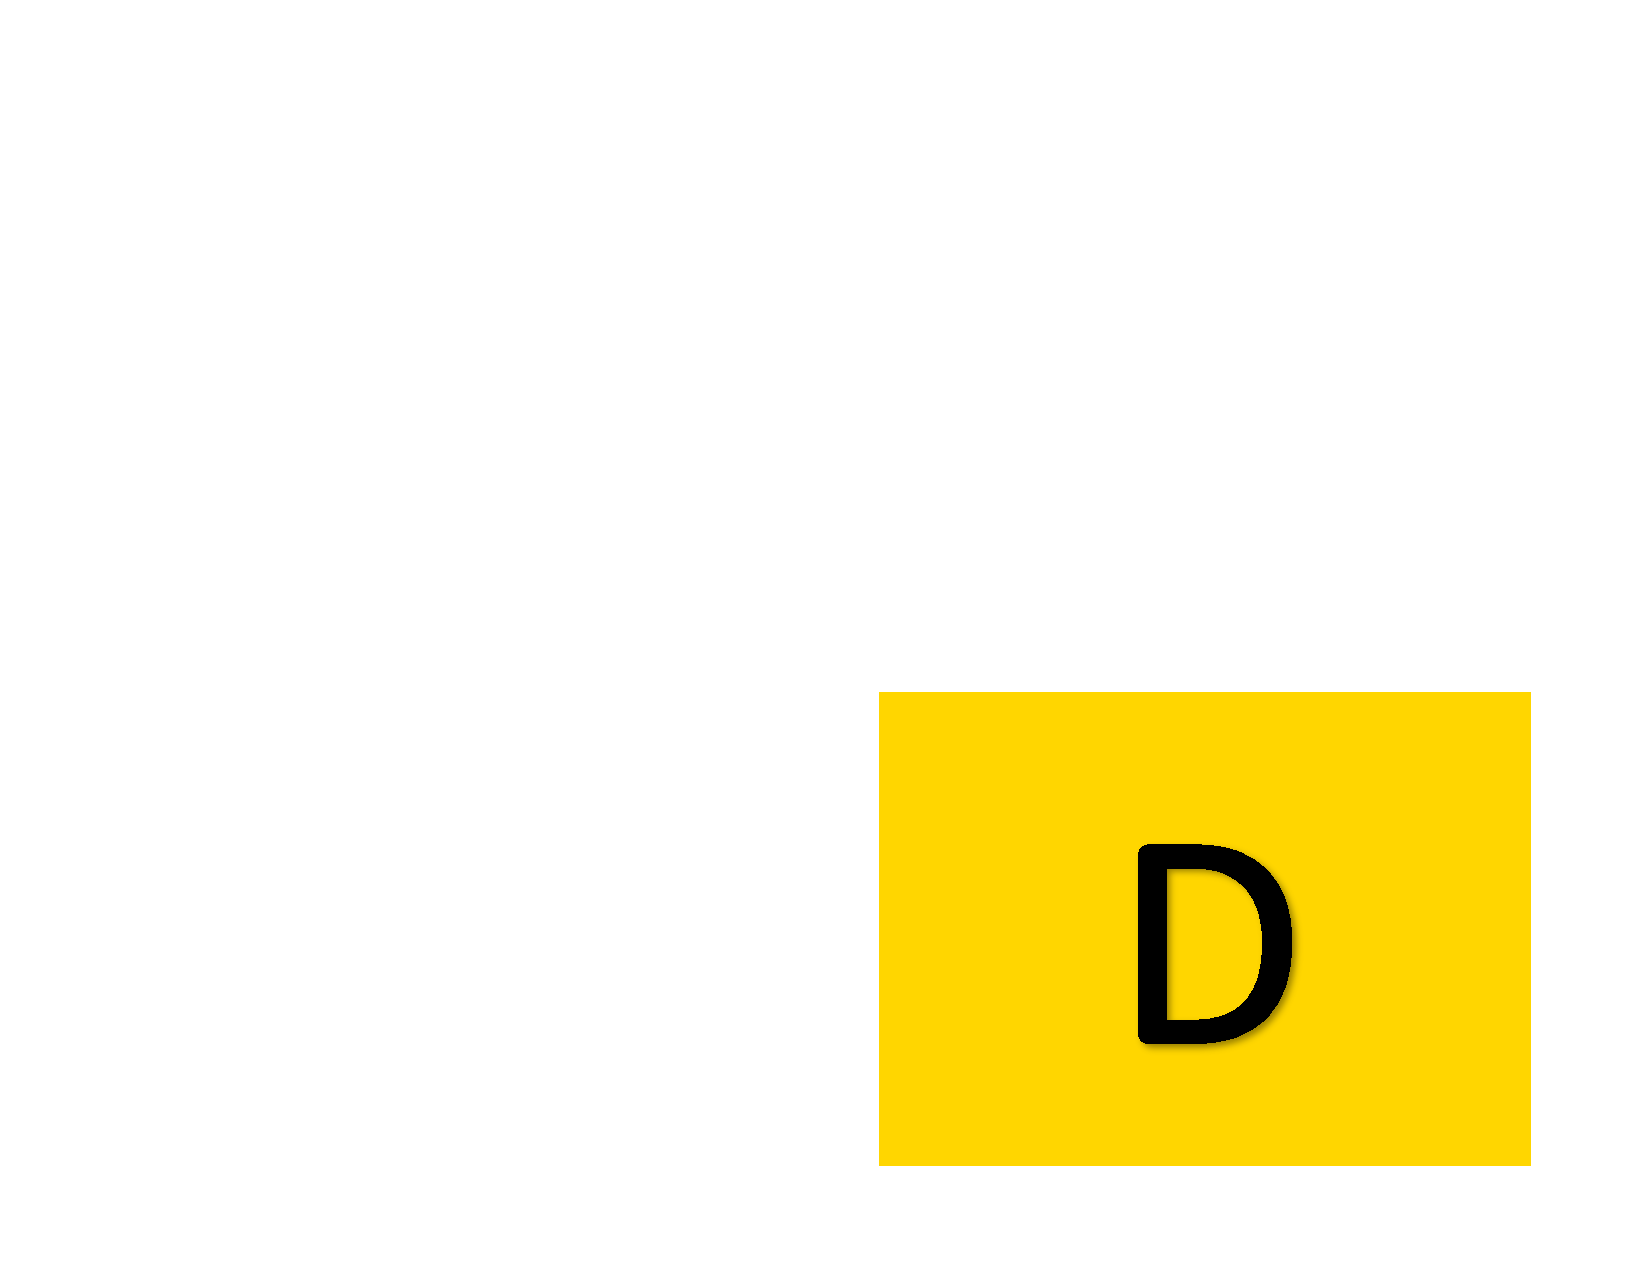
\includegraphics[width=0.8cm,height=0.5cm]{figures/D}} ]  }
\newcommand*{\eitem}{ \item[{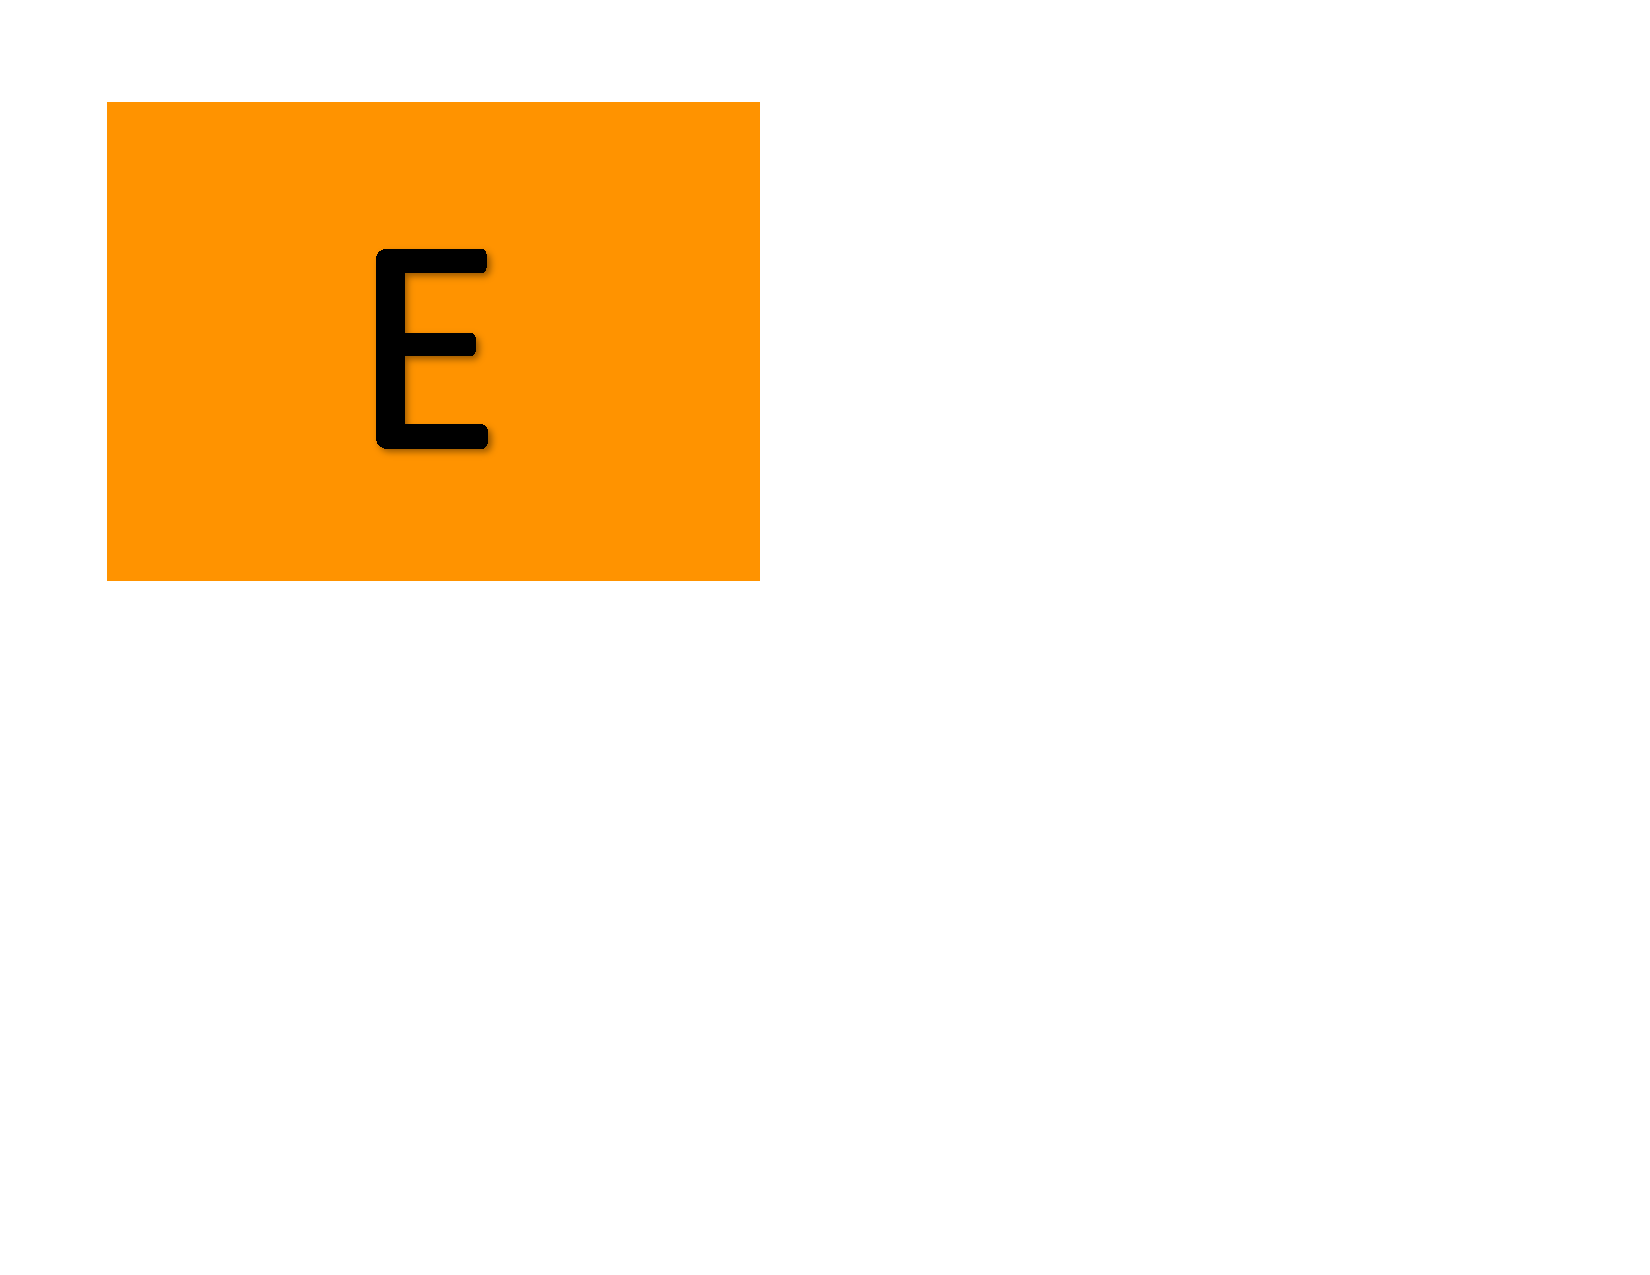
\includegraphics[width=0.8cm,height=0.5cm]{figures/E}} ]  }
\newcommand*{\fitem}{ \item[{
\includegraphics[width=0.8cm,height=0.5cm]{figures/F}} ]  }


\newcommand{\hide}[1]{\underline{\phantom{#1 #1}}}

\usepackage{setspace}

\onehalfspacing
\usepackage{tikz}
\usetikzlibrary{arrows.meta,positioning,calc}

\begin{document}
% Fill in the date when scheduling this lecture.
\sweek{14b: PageRank and Random Walks}{November 12}

% Suggested two-hour plan, including a five-minute break.
% 0--10: Ranking webpages and the limitations of counting links.
% 10--17: The random surfer and the Markov property in words.
% 17--25: Weather example and a two-step probability calculation.
% 25--35: Distribute scores on the running three-page graph.
% 35--45: Check an equilibrium and interpret stationary scores.
% 45--55: Dead ends, traps, and oscillation.
% 55--60: Break.
% 60--72: Teleportation and its qualitative guarantee.
% 72--87: Two PageRank rounds by hand; compare intermediate rankings.
% 87--102: Implement the update and analyze its running time.
% 102--110: Work through a dangling-node example.
% 110--116: Paired exercise: add a link and recompute one round.
% 116--120: Personalization, interpretation, and exit questions.
% This plan includes board work and student discussion. The hand calculations
% and graph-modification exercise supply practice rather than additional theory.
% No matrix notation or general Markov-chain convergence theorem is required.

\section{Ranking Webpages}
Suppose a search engine finds one million pages containing the word
\texttt{university}. Which pages should it display first?

Text matching tells us whether a page mentions a topic. Links provide another
kind of information: which pages other pages refer to.

\paragraph{A first idea: count incoming links}
Why might a page with many incoming links be useful? Can you think of a way
to make this rule give a misleading ranking?
\vs{1.2cm}
% Answer: Incoming links can indicate attention or usefulness, but someone
% could create many low-quality pages that all link to the same target.

\paragraph{Not all links should count equally}
PageRank uses two ideas:
\begin{itemize}
    \item A link from an important page should contribute \hide{more.}
    \vs{.3cm}
    \item More outgoing links divide a page's contribution among
    \hide{more destinations.}
\end{itemize}

The difficulty is that we seem to need to know which pages are important
before we can determine which pages are important.

\begin{Qu}
    How could we get started without knowing the final scores?
    \begin{itemize}
        \aitem Give every page an initial score and repeatedly update the scores
        \bitem Choose the most important page in advance
        \citem Ignore all outgoing links
    \end{itemize}
\end{Qu}
% Answer: (a). We will turn this into a precise iterative algorithm.

\vfill
We will represent the web as a directed graph, define an update rule, and
analyze an algorithm that applies that rule efficiently.

\newpage
\section{A Random Surfer}
Imagine a person browsing the web. At each page, the person chooses one
outgoing link uniformly at random and follows it.

\paragraph{A local rule}
If a page has four outgoing links, the probability of following any particular
one is \hide{$1/4$.} To choose the next page, the surfer only needs to know
\hide{the current page and its outgoing links.}

\begin{center}
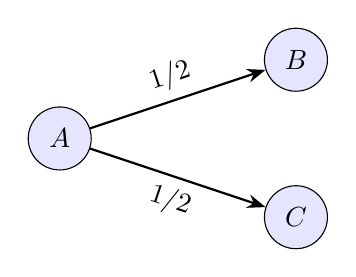
\begin{tikzpicture}[page/.style={circle,draw,fill=blue!10,minimum size=.8cm},
    edge/.style={->,>=Stealth,thick}]
    \node[page] (a) at (0,0) {$A$};
    \node[page] (b) at (3,1) {$B$};
    \node[page] (c) at (3,-1) {$C$};
    \draw[edge] (a)--node[above,sloped] {$1/2$} (b);
    \draw[edge] (a)--node[below,sloped] {$1/2$} (c);
\end{tikzpicture}
\end{center}

\paragraph{The Markov property}
A \textbf{Markov chain} is a random process in which the next-state
probabilities depend only on the current state. They do not require the
entire history of how we arrived there.

For our surfer, the states are \hide{webpages.} We assume that the graph and
the transition rule stay fixed while we analyze the walk.

\begin{Qu}
    Two surfers reach the same page by different routes. Under our rule,
    do they have the same probabilities for their next page?
    \begin{itemize}
        \aitem Yes
        \bitem No, because their browsing histories differ
    \end{itemize}
\end{Qu}
% Answer: (a). The current page determines the available links and their
% probabilities. The two surfers need not make the same random choice.

\vfill
The ranking idea is to give a high score to a page that the surfer visits
often. First, we need a way to keep track of the surfer's probabilities.

\newpage
\subsection*{A small Markov-chain example}
Suppose we use the following simplified model of weather:
\begin{itemize}
    \item After a sunny day, tomorrow is sunny with probability $0.8$.
    \item After a rainy day, tomorrow is sunny with probability $0.4$.
\end{itemize}
This is a model for the example, not a claim that real weather depends only
on whether today is sunny or rainy.

\begin{center}
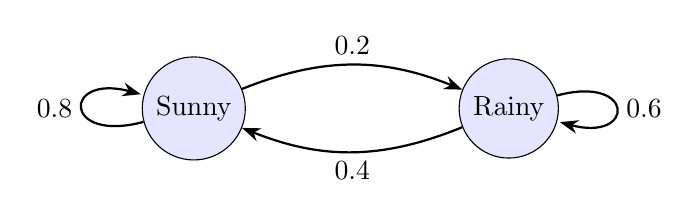
\begin{tikzpicture}[state/.style={circle,draw,fill=blue!10,minimum size=1.1cm},
    edge/.style={->,>=Stealth,thick}]
    \node[state] (s) at (0,0) {Sunny};
    \node[state] (r) at (4,0) {Rainy};
    \draw[edge] (s) to[bend left=22] node[above] {$0.2$} (r);
    \draw[edge] (r) to[bend left=22] node[below] {$0.4$} (s);
    \draw[edge] (s) edge[loop left] node[left] {$0.8$} (s);
    \draw[edge] (r) edge[loop right] node[right] {$0.6$} (r);
\end{tikzpicture}
\end{center}

\paragraph{Predict one day ahead}
If today is sunny, tomorrow's probabilities are
\begin{equation*}
    \Pr[\text{sunny tomorrow}]=\hide{0.8},\qquad
    \Pr[\text{rainy tomorrow}]=\hide{0.2}.
\end{equation*}

\paragraph{Predict two days ahead}
There are two ways to be sunny two days from now:
\begin{itemize}
    \item Sunny tomorrow, then sunny again: probability \hide{$0.8\cdot0.8$.}
    \item Rainy tomorrow, then sunny: probability \hide{$0.2\cdot0.4$.}
\end{itemize}
Adding gives
\begin{equation*}
    \Pr[\text{sunny in two days}]=\hide{0.72}.
\end{equation*}
What is the probability of rain in two days?
\vs{.7cm}
% Answer: 1-0.72=0.28.

\paragraph{Why is this useful?}
A simple rule for one step lets us predict later behavior. Similar models
describe movement through a network, customer queues, and machine operating
states, when the chosen state includes the information needed for the next step.

\vfill
For PageRank, we will perform the same kind of calculation: multiply along
each possible transition, then add the contributions arriving at a page.

\newpage
\section{Distributing Scores Along Links}
We will use the following graph throughout the lecture:
\begin{center}
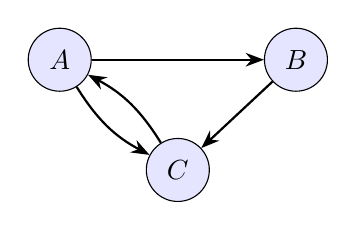
\begin{tikzpicture}[page/.style={circle,draw,fill=blue!10,minimum size=.8cm},
    edge/.style={->,>=Stealth,thick}]
    \node[page] (a) at (0,0) {$A$};
    \node[page] (b) at (3,0) {$B$};
    \node[page] (c) at (1.5,-1.4) {$C$};
    \draw[edge] (a)--(b);
    \draw[edge] (a) to[bend right=15] (c);
    \draw[edge] (b)--(c);
    \draw[edge] (c) to[bend right=15] (a);
\end{tikzpicture}
\end{center}

Let $p(u)$ be the probability that the surfer is currently at page $u$.
The probabilities sum to $1$. We also call these values the current scores.

\paragraph{First, decide what each page sends}
Write $\deg^+(u)$ for the number of outgoing links from $u$. Each outgoing
link receives a contribution of
\begin{equation*}
    \hide{\frac{p(u)}{\deg^+(u)}}.
\end{equation*}
For now, every page has at least one outgoing link.

\paragraph{Next, add what each page receives}
Start with $p(A)=p(B)=p(C)=1/3$. Fill in the new scores:
\begin{equation*}
    p_{\mathrm{new}}(A)=\hide{1/3},\qquad
    p_{\mathrm{new}}(B)=\hide{1/6},\qquad
    p_{\mathrm{new}}(C)=\hide{1/2}.
\end{equation*}
% Answer: C sends 1/3 to A. A sends 1/6 each to B and C.
% B sends its full 1/3 to C, so C receives 1/6+1/3=1/2.

Check that the new scores still sum to $1$. Then perform one more round.
\vs{1.2cm}
% Answer: The second round gives (1/2,1/6,1/3), in the order (A,B,C).

\vfill
All contributions in a round must use the \hide{old scores.} We should not
use a newly computed score until the next round.

\newpage
\subsection*{When have the scores settled down?}
The link-following update is
\begin{equation*}
    p_{\mathrm{new}}(v)=\sum_{u:u\to v}\frac{p(u)}{\deg^+(u)}.
\end{equation*}
A set of probabilities that is unchanged by this update is called a
\textbf{stationary distribution}.

\paragraph{Check a proposed answer}
For our three-page graph, suppose
\begin{equation*}
    p(A)=\frac25,\qquad p(B)=\frac15,\qquad p(C)=\frac25.
\end{equation*}
Without solving any equations, check what happens after another round:
\begin{itemize}
    \item $A$ receives \hide{$2/5$} from $C$.
    \vs{.3cm}
    \item $B$ receives \hide{$1/5$} from $A$.
    \vs{.3cm}
    \item $C$ receives \hide{$1/5+1/5=2/5$} from $A$ and $B$.
\end{itemize}
The probabilities are unchanged, even though the surfer continues moving.

\begin{Qu}
    Pages $A$ and $B$ each have one incoming link. Must they have the same score?
    \begin{itemize}
        \aitem Yes, the number of incoming links determines the score
        \bitem No, the contributions depend on which pages link to them
    \end{itemize}
\end{Qu}
% Answer: (b). Here C sends all of its score to A, while A splits its
% score between B and C.

\paragraph{What does stationary mean?}
Does it mean that the surfer eventually stops at one page?
\vs{.8cm}
% Answer: No. The probability of each page stays the same after an update;
% the actual page visited by an individual surfer can change.

\vfill
This example has sensible stationary scores. Unfortunately, following links
alone does not always give a useful ranking or an iteration that settles down.

\newpage
\section{Why Following Links Is Not Enough}
\paragraph{Dead ends}
Suppose the only link is $A\to B$, and $B$ has no outgoing links. What should
the surfer do after reaching $B$?
\vs{.8cm}
% Answer: The link-following rule gives no next move. Such a page is called
% a dangling node. We will choose a fresh page when this happens.

In score updates, simply discarding the score at $B$ would make the total
score \hide{smaller than $1$.}

\paragraph{Spider traps}
Now consider this graph:
\begin{center}
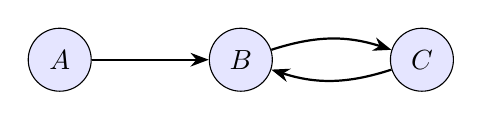
\begin{tikzpicture}[page/.style={circle,draw,fill=blue!10,minimum size=.8cm},
    edge/.style={->,>=Stealth,thick}]
    \node[page] (a) at (0,0) {$A$};
    \node[page] (b) at (2.3,0) {$B$};
    \node[page] (c) at (4.6,0) {$C$};
    \draw[edge] (a)--(b);
    \draw[edge] (b) to[bend left=18] (c);
    \draw[edge] (c) to[bend left=18] (b);
\end{tikzpicture}
\end{center}
Once the surfer enters $\{B,C\}$, it \hide{cannot leave.} A closed group of
pages like this is called a \textbf{spider trap}.

Why might a group receive too much importance just because it links only
to itself?
\vs{.8cm}
% Answer: It retains every surfer who enters, regardless of whether the
% pages are useful or have broad support from the rest of the graph.

\paragraph{Scores can also oscillate}
With just two links $A\to B$ and $B\to A$, start with scores $(1,0)$.
What are the next three pairs of scores?
\vs{.8cm}
% Answer: (0,1), (1,0), (0,1). A stationary pair (1/2,1/2) exists,
% but these updates do not approach it from the chosen start.

\vfill
We need a rule that lets the surfer leave a page or a group of pages without
depending entirely on the available links.
% Suggested five-minute break here.

\newpage
\section{PageRank: Add Random Jumps}
Choose a number $d$ with $0<d<1$. At a page that has outgoing links:
\begin{itemize}
    \item With probability $d$, follow a uniformly chosen outgoing link.
    \item With probability $1-d$, jump to a uniformly chosen page.
\end{itemize}
At a page with no outgoing links, always jump to a uniformly chosen page.
A jump may choose the current page again.

\paragraph{The random-surfer interpretation}
The jumps are called \textbf{teleportation}. For example, if $d=0.85$, the
surfer follows a link with probability \hide{$0.85$} and chooses a random page
with probability \hide{$0.15$}, when outgoing links exist.

\begin{Qu}
    Why can a surfer now escape a spider trap?
    \begin{itemize}
        \aitem We delete the links inside the trap
        \bitem A random jump can move to a page outside the trap
        \citem Every trapped page must gain a new ordinary link
    \end{itemize}
\end{Qu}
% Answer: (b). The same mechanism also connects separate parts of the graph.

\paragraph{The update when there are no dead ends}
If there are $n$ pages, then
\begin{equation*}
    p_{\mathrm{new}}(v)=\frac{1-d}{n}
      +d\sum_{u:u\to v}\frac{p(u)}{\deg^+(u)}.
\end{equation*}
The first term is the contribution from \hide{random jumps.} The second is
the contribution from \hide{following links.}
% The link-following sum assumes all pages have positive out-degree.
% The general implementation below also redistributes dangling-node mass.

\paragraph{What we can guarantee}
With these jumps and the dead-end rule, there is a unique stationary set of
scores. Repeated updates approach those scores from any starting probability
distribution. We will use this fact without proving it.

\vfill
These stationary scores are the \textbf{PageRank scores}. They describe how
often the modified random surfer visits each page in the long run.

\newpage
\subsection*{Compute two PageRank rounds}
Return to the links $A\to B$, $A\to C$, $B\to C$, and $C\to A$.
Use $d=1/2$ to keep the arithmetic simple, and start with score $1/3$ at each page.

\paragraph{First, add the jump contribution}
There are three pages, so each receives
\begin{equation*}
    \frac{1-d}{3}=\hide{\frac16}.
\end{equation*}

\paragraph{Next, add the link contributions}
For this graph, one round is
\begin{equation*}
    \begin{aligned}
        p_{\mathrm{new}}(A)&=\frac16+\frac12p(C),\\
        p_{\mathrm{new}}(B)&=\frac16+\frac14p(A),\\
        p_{\mathrm{new}}(C)&=\frac16+\frac14p(A)+\frac12p(B).
    \end{aligned}
\end{equation*}
Why is the coefficient of $p(A)$ equal to $1/4$ rather than $1/2$?
\vs{.6cm}
% Answer: A splits its score between two links, and the probability of
% following a link is 1/2. Each contribution is (1/2)(p(A)/2)=p(A)/4.

\paragraph{Fill in the table}
\begin{center}
\renewcommand{\arraystretch}{1.7}
\begin{tabular}{c|ccc}
Round & $A$ & $B$ & $C$\\\hline
0 & $1/3$ & $1/3$ & $1/3$\\
1 & $\hide{1/3}$ & $\hide{1/4}$ & $\hide{5/12}$\\
2 & $\hide{3/8}$ & $\hide{1/4}$ & $\hide{3/8}$
\end{tabular}
\end{center}
Check that each row sums to $1$. Which page is ranked first after each round?
\vs{.6cm}
% Answer: C is first after round 1. A and C tie after round 2.

\vfill
After many rounds, the scores approach approximately $(0.359,0.256,0.385)$,
so the final ordering is $C>A>B$. A small number of rounds need not give
the final ordering, especially when scores are close.
% The exact stationary scores are (14,10,15)/39. They may be checked by
% substitution, but solving the three simultaneous equations is not required.

\newpage
\section{Implementing the Algorithm}
We can compute all the new scores by scanning the outgoing links of each
page. Store the graph using adjacency lists.

\paragraph{Remember the pages with no outgoing links}
Let $z$ be the sum of their current scores. In addition to the ordinary jump
contribution, distribute their remaining score $dz$ uniformly. Thus each
page starts the round with $((1-d)+dz)/n$.

\begin{algorithm}[h]
    \textsc{PageRank}($G,d,K$), where $0<d<1$ and $K\geq1$
    \begin{algorithmic}
        \State Let $n=|V|$ and compute the out-degree $\deg^+(u)$ of every page
        \State Initialize $p(u)\gets1/n$ for every page $u$
        \For{$t=1,\ldots,K$}
            \State $z\gets\sum_{u:\deg^+(u)=0}p(u)$
            \State $p_{\mathrm{new}}(v)\gets((1-d)+dz)/n$ for every page $v$
            \For{each edge $(u,v)\in E$}
                \State $p_{\mathrm{new}}(v)\gets p_{\mathrm{new}}(v)+d\,p(u)/\deg^+(u)$
            \EndFor
            \State $p\gets p_{\mathrm{new}}$
        \EndFor
        \State \Return $p$
    \end{algorithmic}
\end{algorithm}

\paragraph{Why use two arrays?}
Why should we not overwrite $p(v)$ immediately as we scan the edges?
\vs{.7cm}
% Answer: Every contribution must use the same old scores. Otherwise an
% updated page could send its new score during the current round, making
% the result depend on the order in which we scan edges.

\begin{Qu}
    What is the running time of one round?
    \begin{itemize}
        \aitem $O(n+|E|)$
        \bitem $O(n^2)$, because a jump can go to any page
        \citem $O(|E|^2)$
    \end{itemize}
\end{Qu}
% Answer: (a). Scan the vertices for dangling mass and initialization,
% and scan the edges once. We never explicitly create all possible jump edges.

With $K$ rounds, the total running time is \hide{$O(K(n+|E|))$.}
The two score arrays use $O(n)$ space in addition to the graph.
The returned scores after $K$ rounds are approximations.
% K is a positive integer. The output is an approximation; we are not
% claiming an accuracy guarantee for an arbitrary chosen value of K.

\newpage
\subsection*{Check the dead-end rule}
Suppose there are only two pages, with the single link $A\to B$.
Page $B$ has no outgoing links. Start with $p(A)=p(B)=1/2$, and use $d=1/2$.

\paragraph{Follow what happens to the score at $A$}
Half of $A$'s score follows its link to $B$. The other half is split equally
between the two pages by random jumps.
\begin{equation*}
    \text{From $A$ to $A$: }\hide{\frac18},\qquad
    \text{from $A$ to $B$: }\hide{\frac38}.
\end{equation*}

\paragraph{Follow what happens to the score at $B$}
There is no outgoing link, so all of $B$'s score is distributed uniformly:
\begin{equation*}
    \text{From $B$ to $A$: }\hide{\frac14},\qquad
    \text{from $B$ to $B$: }\hide{\frac14}.
\end{equation*}

\paragraph{Add the contributions}
The new scores are
\begin{equation*}
    p_{\mathrm{new}}(A)=\hide{\frac38},\qquad
    p_{\mathrm{new}}(B)=\hide{\frac58}.
\end{equation*}
Check that their sum is $1$.

\paragraph{Now compare with the algorithm}
Here $z=\hide{1/2}$, so the initialization gives every page
\begin{equation*}
    \frac{(1-d)+dz}{2}=\hide{\frac38}.
\end{equation*}
The edge $A\to B$ then adds \hide{$1/4$} to $B$.

\begin{Qu}
    What would go wrong if we initialized each score to $(1-d)/2$ and
    then scanned the edges, without accounting for $z$?
\end{Qu}
\vs{1cm}
% Answer: We would get (1/4,1/2), whose entries sum to only 3/4.
% We lost the half of B's score assigned to the link-follow option.

\vfill
Every page must distribute all of its score. Having no outgoing links is a
case the implementation must handle explicitly.

\newpage
\section{What Happens If We Add a Link?}
Work with a partner. Start with our original three-page graph, then add the
link $B\to A$. The new graph is shown below.

\begin{center}
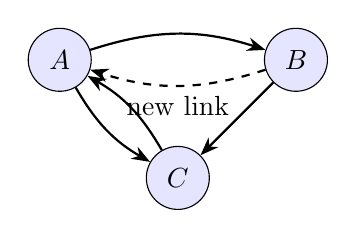
\begin{tikzpicture}[page/.style={circle,draw,fill=blue!10,minimum size=.8cm},
    edge/.style={->,>=Stealth,thick}]
    \node[page] (a) at (0,0) {$A$};
    \node[page] (b) at (3,0) {$B$};
    \node[page] (c) at (1.5,-1.5) {$C$};
    \draw[edge] (a) to[bend left=18] (b);
    \draw[edge,dashed] (b) to[bend left=18] node[below] {new link} (a);
    \draw[edge] (a) to[bend right=15] (c);
    \draw[edge] (b)--(c);
    \draw[edge] (c) to[bend right=15] (a);
\end{tikzpicture}
\end{center}

Use $d=1/2$ and restart the calculation with score $1/3$ at each page.

\paragraph{Predict before calculating}
Which page receives a new contribution? Which old contribution becomes smaller?
\vs{1cm}
% Answer: A now receives a contribution from B. B splits its link-following
% score between A and C, so the contribution from B to C becomes smaller.

\paragraph{Compute one round}
\begin{equation*}
    p_{\mathrm{new}}(A)=\hide{\frac5{12}},\qquad
    p_{\mathrm{new}}(B)=\hide{\frac14},\qquad
    p_{\mathrm{new}}(C)=\hide{\frac13}.
\end{equation*}
Compare this with the old first-round scores $(1/3,1/4,5/12)$.

\paragraph{Explain the change}
Page $C$ still has the same two incoming links. Why did its score decrease
in this round?
\vs{.8cm}
% Answer: The source B now divides its contribution between two destinations.
% Counting incoming links alone misses this change in contribution size.

\vfill
This compares one round from the same starting scores. To find the new
stationary ranking, we would continue applying updates on the new graph.

\newpage
\section{Using and Interpreting PageRank}
\paragraph{A score for the graph}
Ordinary PageRank depends on the link graph, not on a particular search
query. We can compute it in advance and combine it with information about
how well each page matches a query.

Would a page with a high PageRank necessarily be a good answer to a search
for a particular restaurant's opening hours?
\vs{.7cm}
% Answer: No. Link-based importance does not imply relevance to the query.
% A small relevant page may be more useful than a highly ranked general page.

\paragraph{Changing the jump rule}
For \textbf{personalized PageRank}, random jumps favor selected pages, such
as pages about a topic or items a user likes. Following links then spreads
that emphasis through the graph.

What might this be useful for besides ranking webpages?
\vs{.7cm}
% Answer: Finding related items for recommendations, identifying papers
% near a research topic, or exploring a user's part of a social network.

\paragraph{Changing $d$}
More frequent jumps make the starting point matter less and put more emphasis
on the jump rule. More link-following makes the graph structure more influential.

If $d=0$ and jumps are uniform, what scores do we obtain?
\vs{.6cm}
% Answer: Every page has score 1/n, regardless of the links. At d=1,
% the original problems with traps and oscillation can return.

\begin{Qu}
    Which statement best describes PageRank?
    \begin{itemize}
        \aitem It counts incoming links
        \bitem It computes scores from a random-surfer model by repeated updates
        \citem It guarantees that highly ranked pages are true and useful
    \end{itemize}
\end{Qu}
% Answer: (b). The model is useful, but links can be manipulated and the
% scores alone do not establish truth, usefulness, or query relevance.

\vfill
The main algorithmic ideas are to model a problem using a graph, define a
local update, and compute repeated updates by scanning vertices and edges.

\end{document}
